% back-nozzle.tex

\newpage
\section{Flow through a conical nozzle}
\label{back-nozzle-sec}
%
Good quality experimental data for wall pressure distribution in a conical
nozzle with a circular-arc throat profile and a 15$^o$ divergent section
is available in Ref.\,\cite{back_etal_1965a}.
In the original experiment the flow of air through the facility 
was allowed to reach steady state and static pressures were measured 
at a large number of points along the nozzle wall.
In contrast, the present simulation is transient with just the transonic 
plus supersonic parts of the flow field reaching steady state.

Figure\,\ref{back-geometry-fig} shows the outline of the simulated flow
domain which is set up to approximate the largest subsonic area ratio
used in the experiment.
Note that the geometric calculation of the tangent arcs is done within the
input script.
This makes use of Python, beyond just being an input format, and allows the
specification to be fully parametric.
This makes the initial setup of the script a bit more complex than absolutely
necessary but does make the running of the simulation for other radii of curvature 
very simple.


The relatively long upstream part of the simulated tube provides the gas 
through an unsteady expansion from zero speed and pressure of 500\,kPa 
(state 4) up to a small Mach number (state 3).
These state labels refer to the those for 
the hypothetical shock tube problem in which 
state 1 is the initial low-pressure condition, 
state 4 is the initial high-pressure condition,
state 2 is the post-shock condition of the low-pressure gas,
and state 3 is the expanded high-pressure gas condition.
Assuming that flow in the subsonic and transonic regions of the nozzle is
steady, the expected Mach number is $M_3 = 0.13812$ for an area ratio of 
$A_3 / A_* = 4.2381$.

\begin{figure}[htbp]
\begin{center}
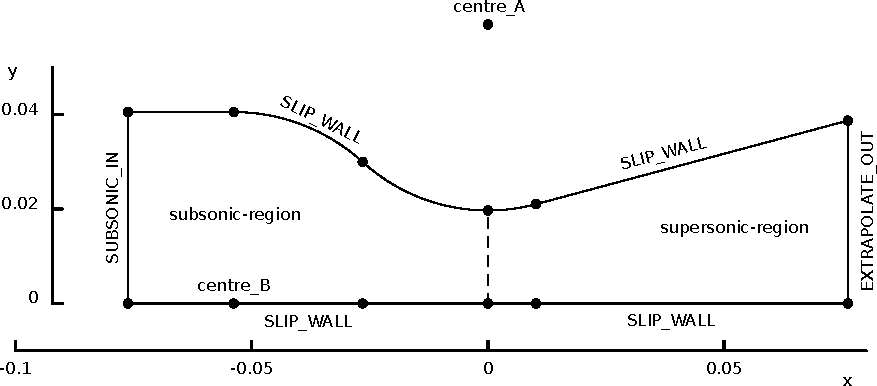
\includegraphics[width=\textwidth,viewport=14 17 439 130,clip=true]{../2D/back-nozzle/back-layout.pdf}
\end{center}
\caption{Schematic diagram of the full flow domain for the duct and conical nozzle.}
\label{back-geometry-fig}
\end{figure}

Along the $C_+$ characteristic connecting states 4 and 3, 
the Riemann invariant can be written as 
$$
    J_+ = u + \frac{2 a}{\gamma - 1} ~~~,
$$
and so the relation between states 4 and 3 can be written as
$$
    \frac{a_4}{a_3} = 1 + \frac{\gamma - 1}{2} M_3 ~~~.
$$
Because the unsteady expansion is isentropic and $a = \sqrt{\gamma R T}$,
the pressure ratio can be written as
$$
    \frac{p_4}{p_3} = \left[ 1 + \frac{\gamma - 1}{2} M_3 
                      \right]^{2 \gamma / (\gamma - 1)}
$$
which gives a specific pressure ratio of $p_4/p_3 = 1.2102$.
Since the experiment used a steady expansion from a large reservoir
at stagnation conditions to the equivalent of our state 3, 
the corresponding stagnation pressure for state 3 is computed from
$$
    \frac{p_{03}}{p_3} = \left[ 1 + \frac{\gamma - 1}{2} M_3^2
                               \right]^{\gamma / (\gamma - 1)} 
$$
which gives $p_{03} = 418.7$\,kPa in the current simulation.

Figure\,\ref{back-mesh-fig} shown part of the mesh around the nozzle
overlaid with pressure contours.
Figure\,\ref{back-pressure-contours-fig} shows the pressure distribution
throughout the flow domain at $t = 1.0$\,ms.
A shock, starting at the transition from circular arc to straight wall
in the early supersonic part of the nozzle, can be seen propagating
toward the centreline as the flow proceeds to the exit plane.

\begin{figure}[htbp]
\begin{center}
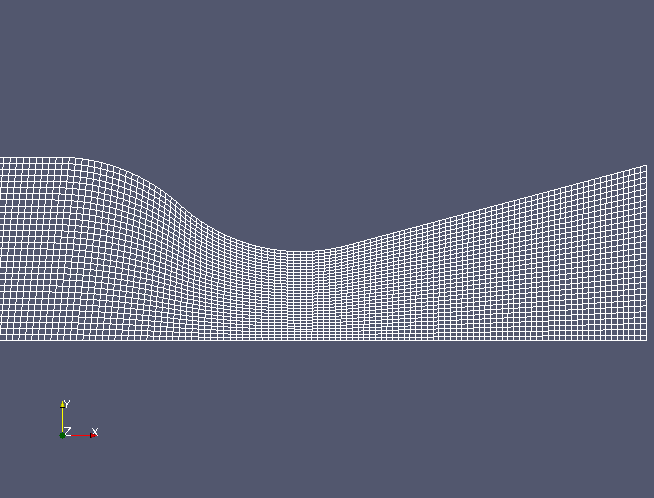
\includegraphics[width=0.8\textwidth]{../2D/back-nozzle/back-mesh.png}
\end{center}
\caption{Downstream-end of the mesh generated for the axisymmetric nozzle simulation.}
\label{back-mesh-fig}
\end{figure}

\begin{figure}[htbp]
\begin{center}
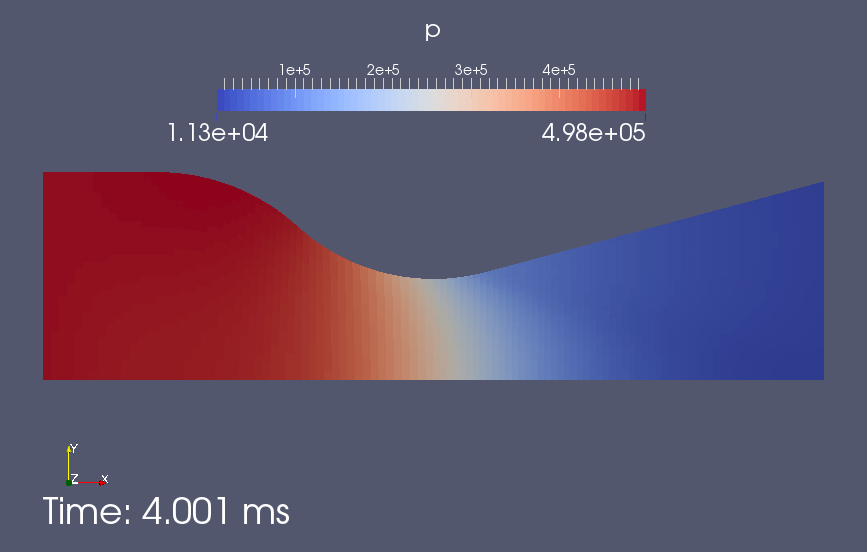
\includegraphics[width=0.8\textwidth]{../2D/back-nozzle/back-p-field.png}
\end{center}
\caption{Pressure contours within the flow domain at 1.0\,ms.}
\label{back-pressure-contours-fig}
\end{figure}

The flow in the nozzle is reasonably steady, as indicated by the histories
shown in Fig.\,\ref{back-transient-fig} but the unsteady expansion can 
be seen reflecting from the inflow boundary at $x = -0.245$\,m 
in Fig.\ref{back-pressure-contours-fig}.

\begin{figure}[htbp]
\begin{center}
\begin{tabular}{cc}
(a) & (b) \\
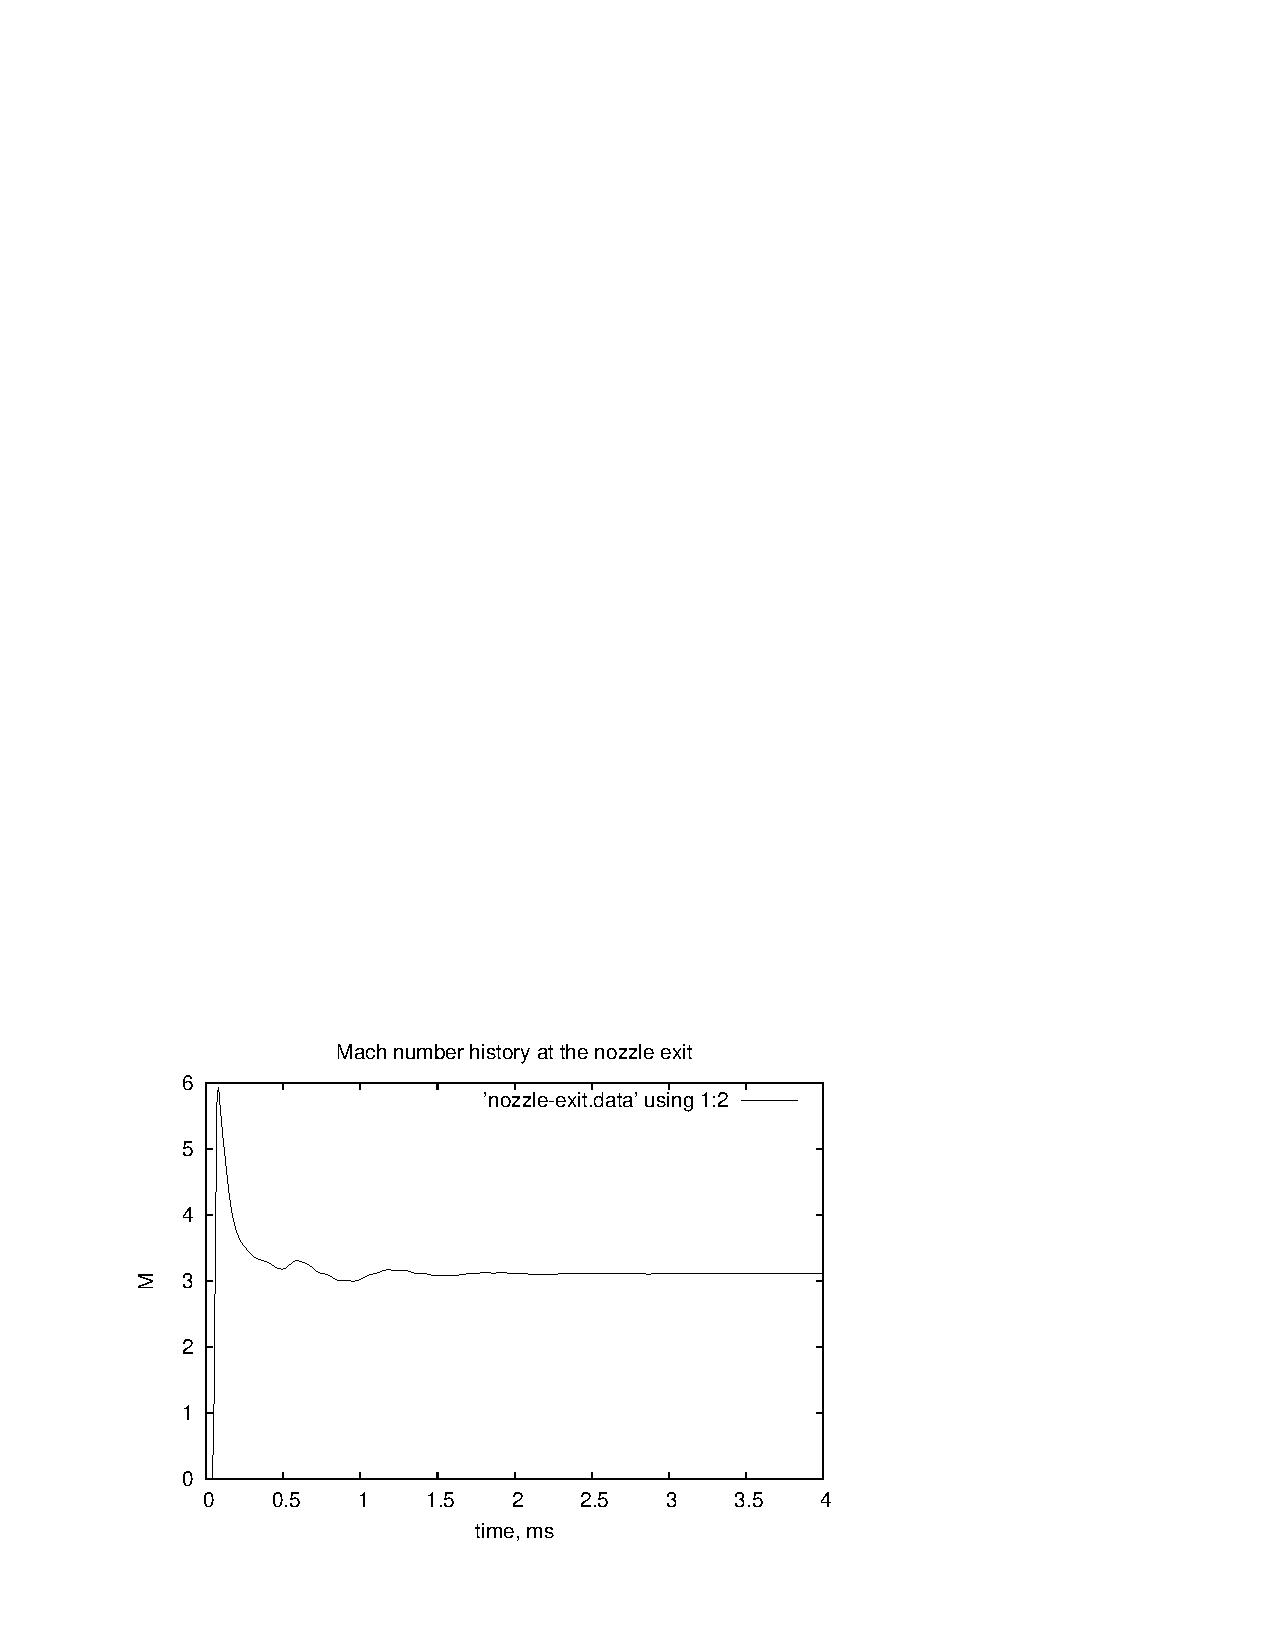
\includegraphics[width=0.5\textwidth,viewport=65 52 398 291,clip=true]{../2D/back-nozzle/back_history_M.pdf} &
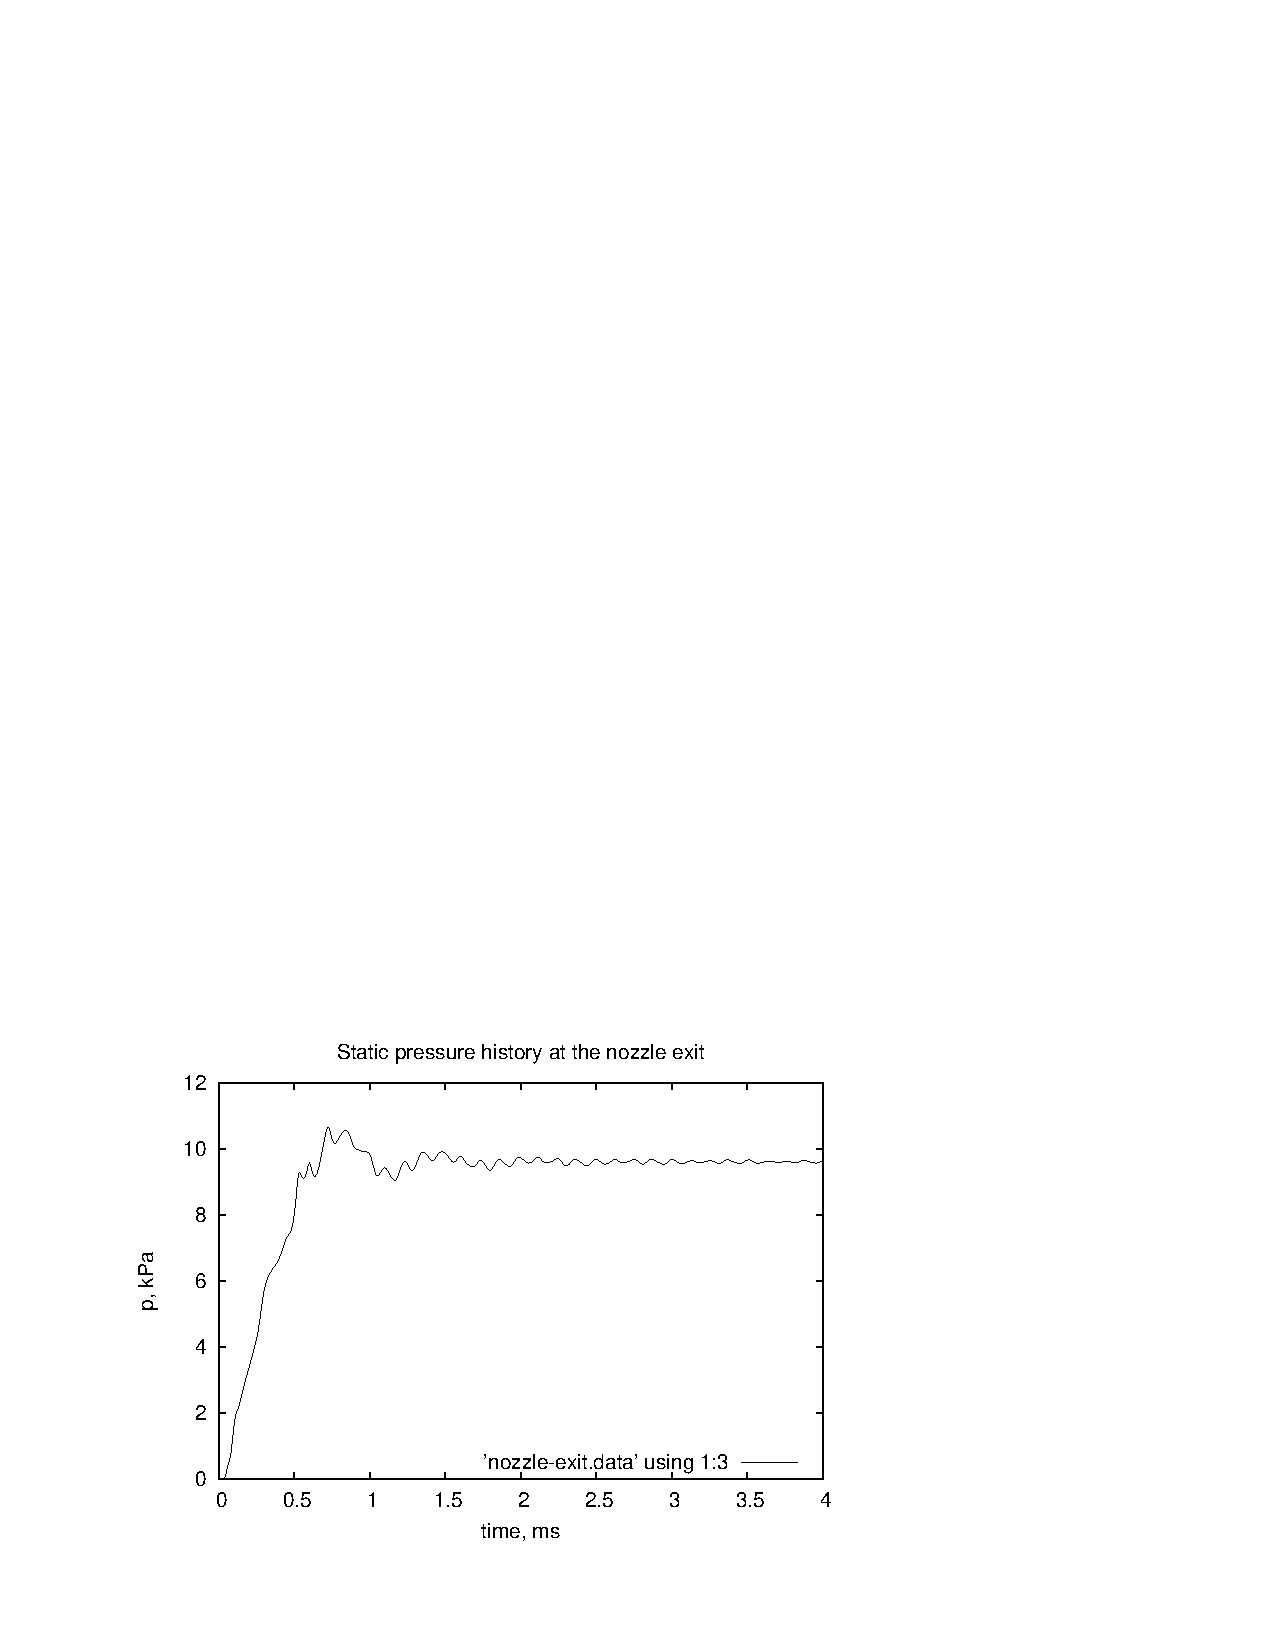
\includegraphics[width=0.5\textwidth,viewport=65 52 398 291,clip=true]{../2D/back-nozzle/back_history_p.pdf}
\end{tabular}
\end{center}
\caption{Development of the flow at a ``history point'' near
         the centre of the exit plane:
         (a) Mach number;
         (b) static pressure.}
\label{back-transient-fig}
\end{figure}

Figure\,\ref{back-profile-fig} shows that the simulation matches the
experimental data closely.
The reflected expansion is shown clearly in the left figure and indicates 
that the subsonic boundary condition is not working as well as it should.


\begin{figure}[htbp]
\begin{center}
\begin{tabular}{cc}
(a) & (b) \\
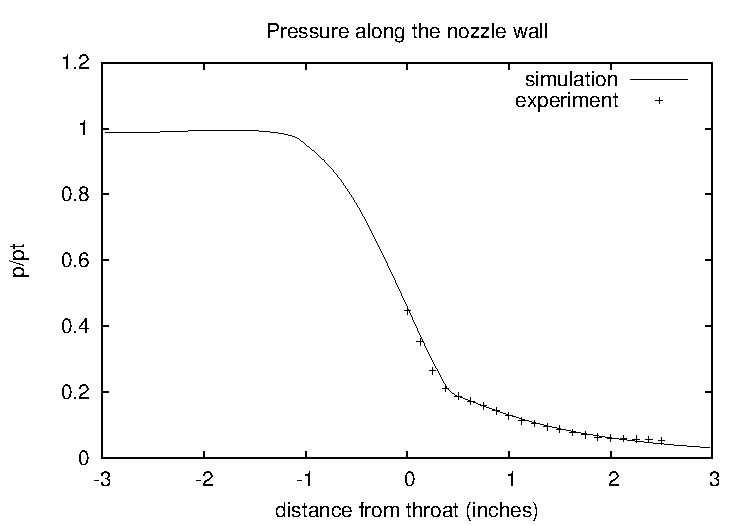
\includegraphics[width=0.5\textwidth,viewport=65 54 398 291,clip=true]{../2D/back-nozzle/back_profile_whole.pdf} &
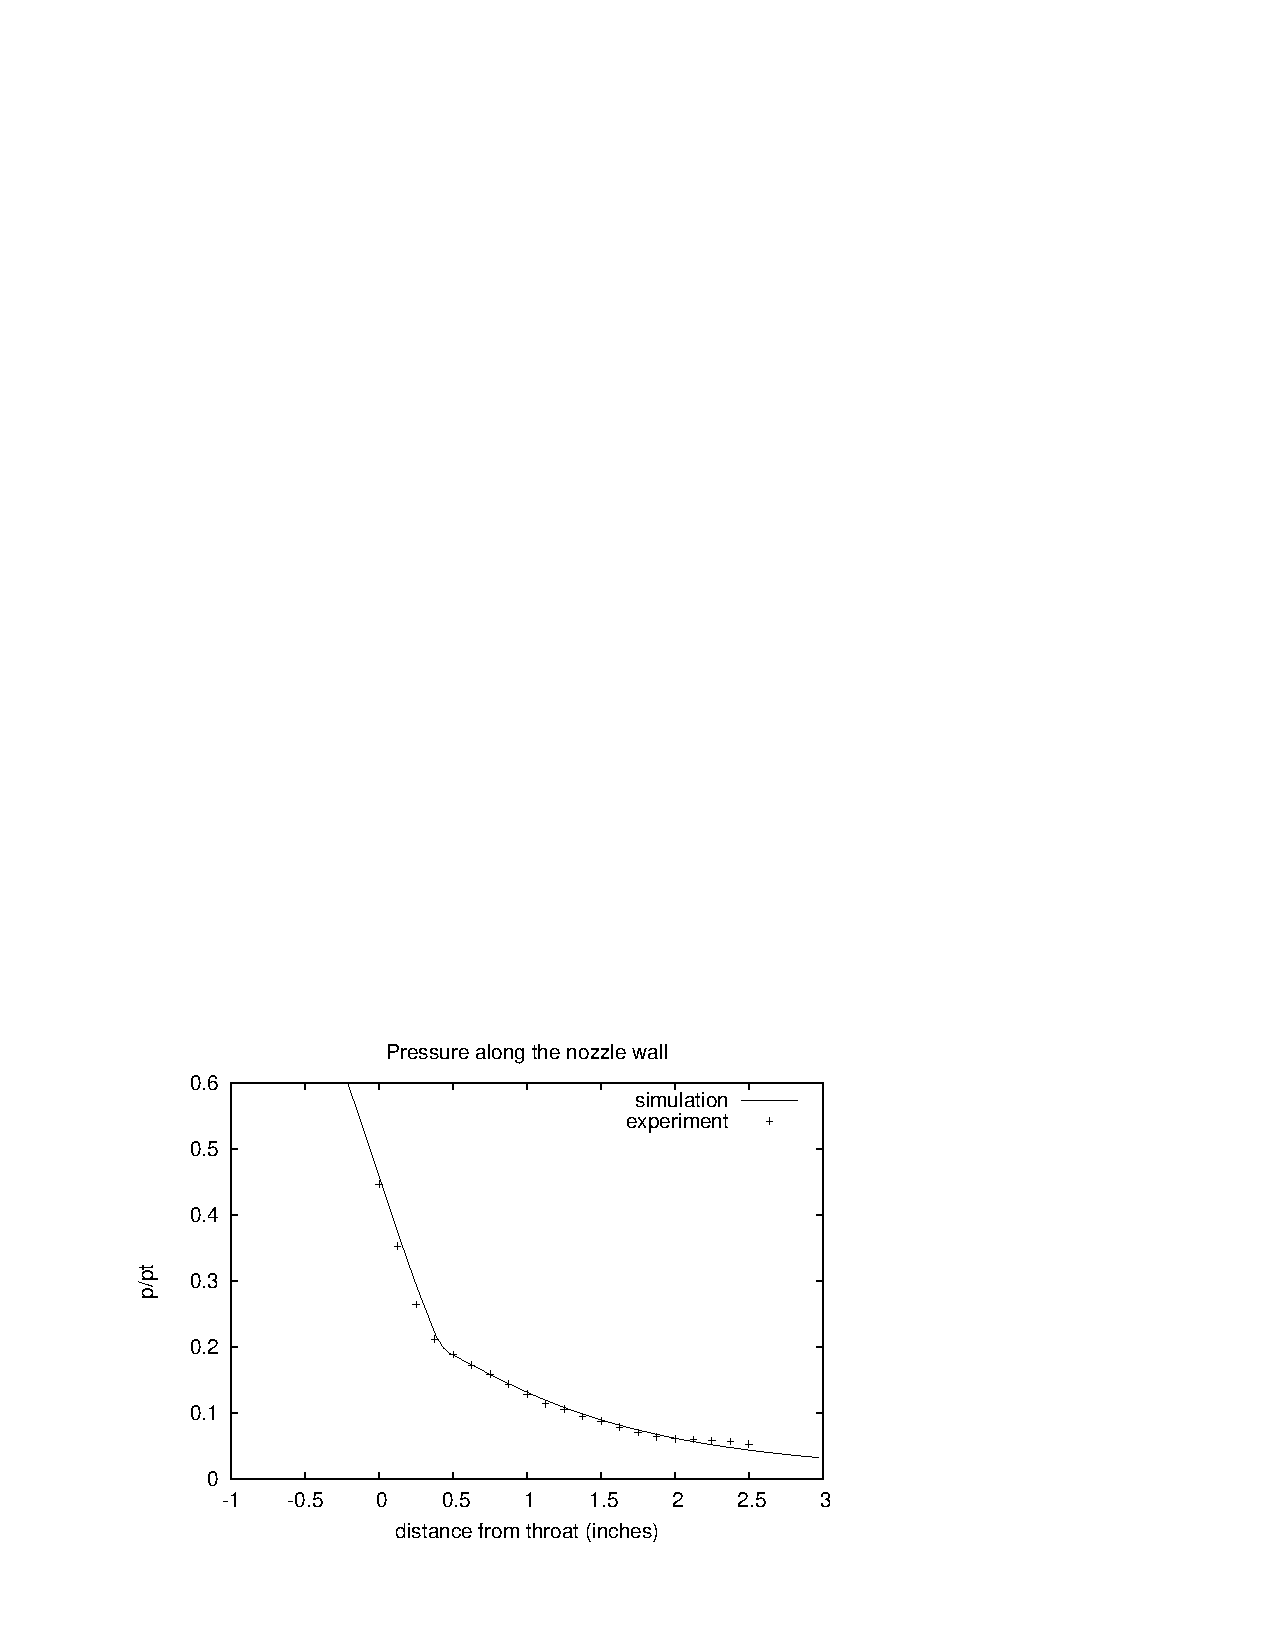
\includegraphics[width=0.5\textwidth,viewport=65 54 398 291,clip=true]{../2D/back-nozzle/back_profile_supersonic.pdf}
\end{tabular}
\end{center}
\caption{Normalised pressure distribution along the nozzle wall:
         (a) full length of flow domain; 
	 (b) just the supersonic part of the nozzle.}
\label{back-profile-fig}
\end{figure}

\newpage
\subsection{Input script (.py)}
\topbar
\lstinputlisting[language={}]{../2D/back-nozzle/back.py}
\bottombar


\subsection{Shell scripts}
\label{back-sh-files}
\topbar
\lstinputlisting[language={}]{../2D/back-nozzle/back_run.sh}
\bottombar

\noindent
\topbar
\lstinputlisting[language={}]{../2D/back-nozzle/back_profile.sh}
\bottombar

\noindent
\topbar
\lstinputlisting[language={}]{../2D/back-nozzle/back_history.sh}\index{history location!extracting the data}
\bottombar

\newpage
\subsection{Notes}
\begin{itemize}
\item The simulation reaches a final time of 1\,ms in 1448 steps and,
      on an Intel E2140 1.60\,Ghz system, this takes 5\,min, 16\,s of CPU time.
\item When run using \texttt{mbcns2}, the simulation reaches a final time of 1\,ms in 1431 steps and,
      on a Pentium-M 1.73\,Ghz system, this takes 2\,min, 50\,s of CPU time.
      This is equivalent to 16.5\,$\mu$s per cell per predictor-corrector
      time step.
\item The pressure is normalised with respect to the stagnation pressure
      using the following AWK script.\\
      \topbarshort
      \lstinputlisting[language={}]{../2D/back-nozzle/normalize.awk}
      \bottombarshort\\
\item The history data for all of the history cells in a particular block are
      written to the one file.
      A particular cell can be extracted as shown by the following AWK script.\\
      \topbarshort
      \lstinputlisting[language={}]{../2D/back-nozzle/extract-history.awk}
      \bottombarshort\\
\end{itemize}
